\documentclass[10pt,a4paper]{article}
\usepackage[utf8]{inputenc}
\usepackage{amsmath}
\usepackage{amsfonts}
\usepackage{amssymb}
\usepackage{graphicx}
\author{Ricardo Arango Giraldo}
\title{Prueba de selección en Rappi}
\begin{document}
\maketitle
	El equipo de operaciones de Rappi está interesado en predecir qué órdenes tienen más probabilidades de ser cancelados ya que no son lo suficientemente atractivos para los mensajeros. Para resolver este problema, tenemos una muestra de pedidos creados en septiembre de 2017.\\
	Su objetivo es utilizar este conjunto de datos para ayudar a Rappi a comprender qué factores influyen si un servicio es tomado y ofrecer recomendaciones para tomar acciones basadas en sus ideas para mejorar la operación de Rappi.
	\section{Exploración}
		La variable \textit{taken} corresponde a la variable objetivo que se quiere predecir. En este caso, la aceptación (o toma) del servicio, esta variable es de carácter booleano. Toma el valor de 1 si la orden fue tomada, 0 en otro caso.\\
		
		\begin{figure}[h]
			\centering
			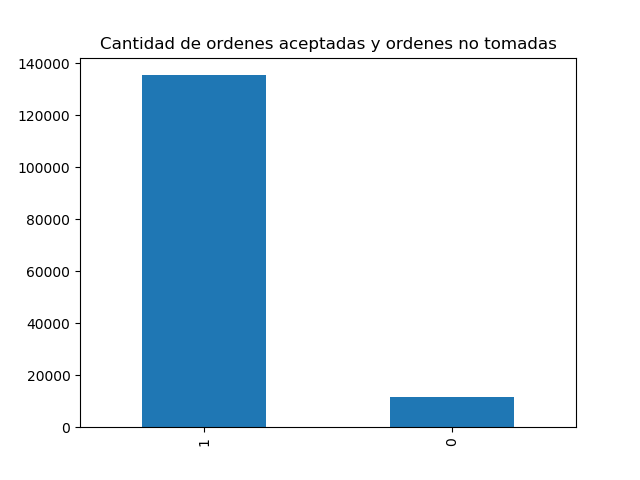
\includegraphics[width=0.5\textwidth]{../Img/Figure_1}
		\end{figure}
		La variable \textit{to\_user\_distance} es de tipo numérica, es decir que su rango son todos los reales y es una variable aleatoria continua. Esta corresponde a la distancia (en km) entre la tienda y la ubicación del usuario.\\
		
		\begin{figure}[h]
			\centering
			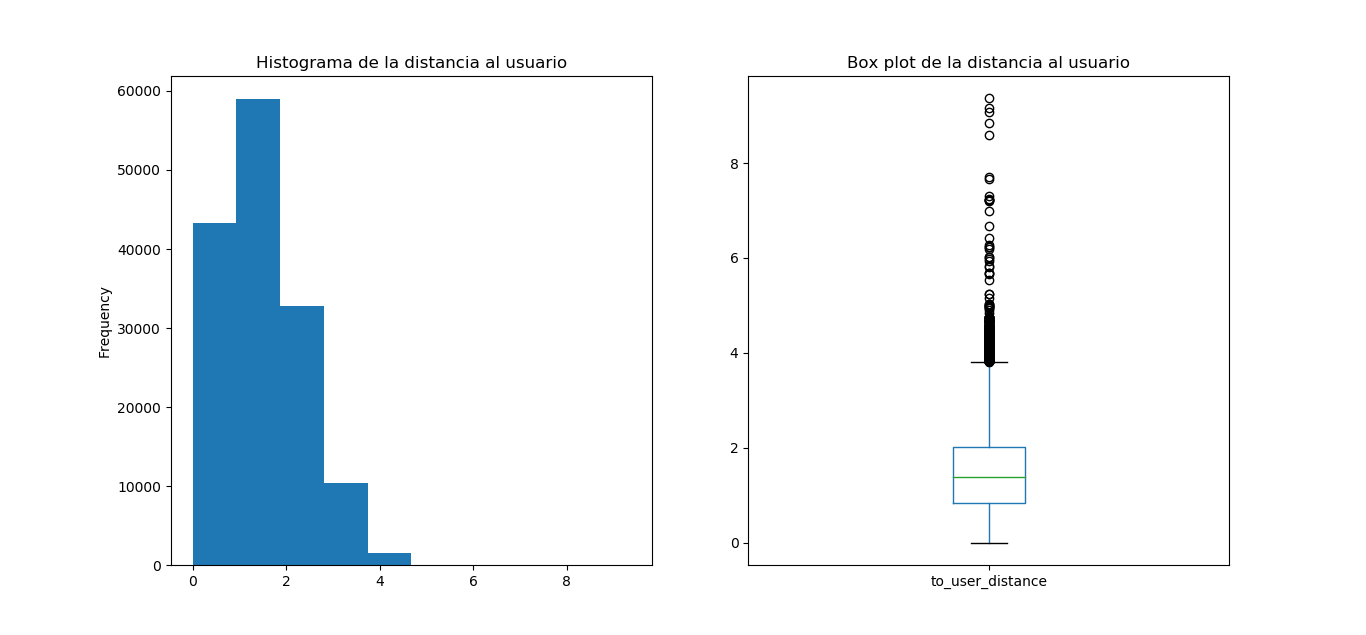
\includegraphics[width=0.5\textwidth]{../Img/to_user_distance}
		\end{figure}
		La variable \textit{to\_user\_elevation} es de tipo numérica, es decir que su rango son todos los reales y es una variable aleatoria continua. Esta corresponde a la diferencia (en metros) entre la tienda y la altitud del usuario.\\
				
		\begin{figure}[h]
			\centering
			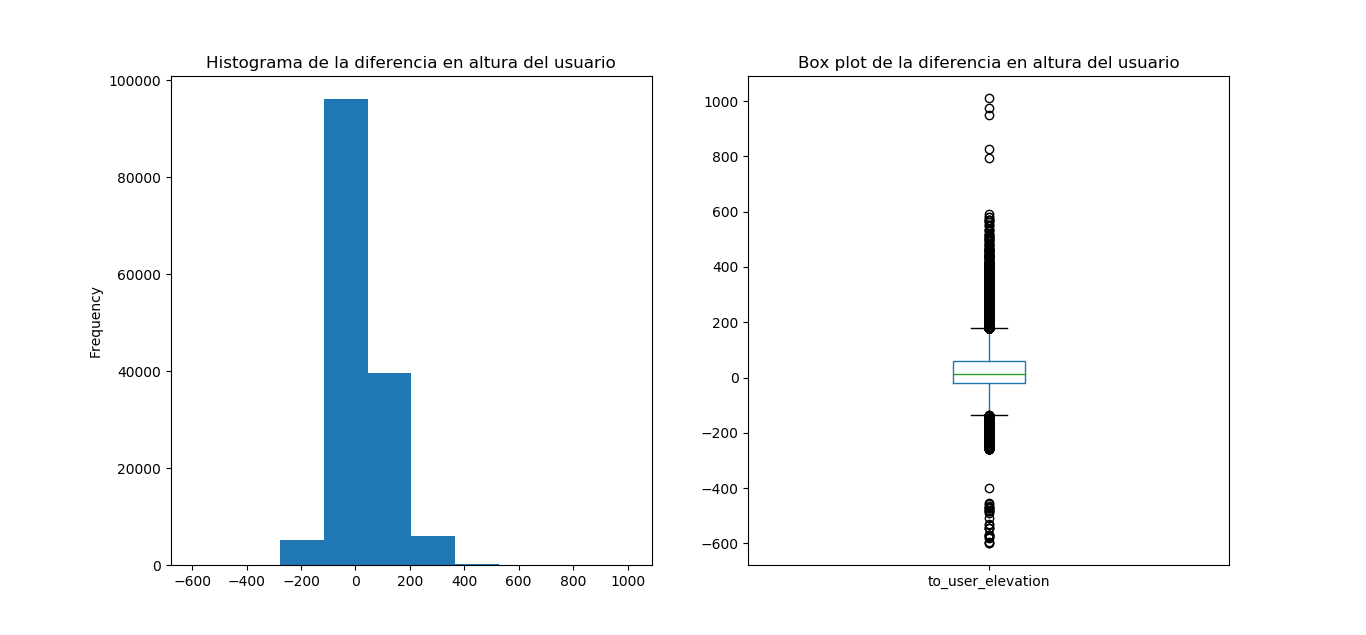
\includegraphics[width=0.5\textwidth]{../Img/to_user_elevation}
		\end{figure}
		La variable \textit{total\_earning} es de tipo numérica, es decir que su rango son todos los reales y es una variable aleatoria continua. Esta corresponde	la ganancia (en pesos colombianos) por la entrega del pedido.\\
		
		\begin{figure}[h]
			\centering
			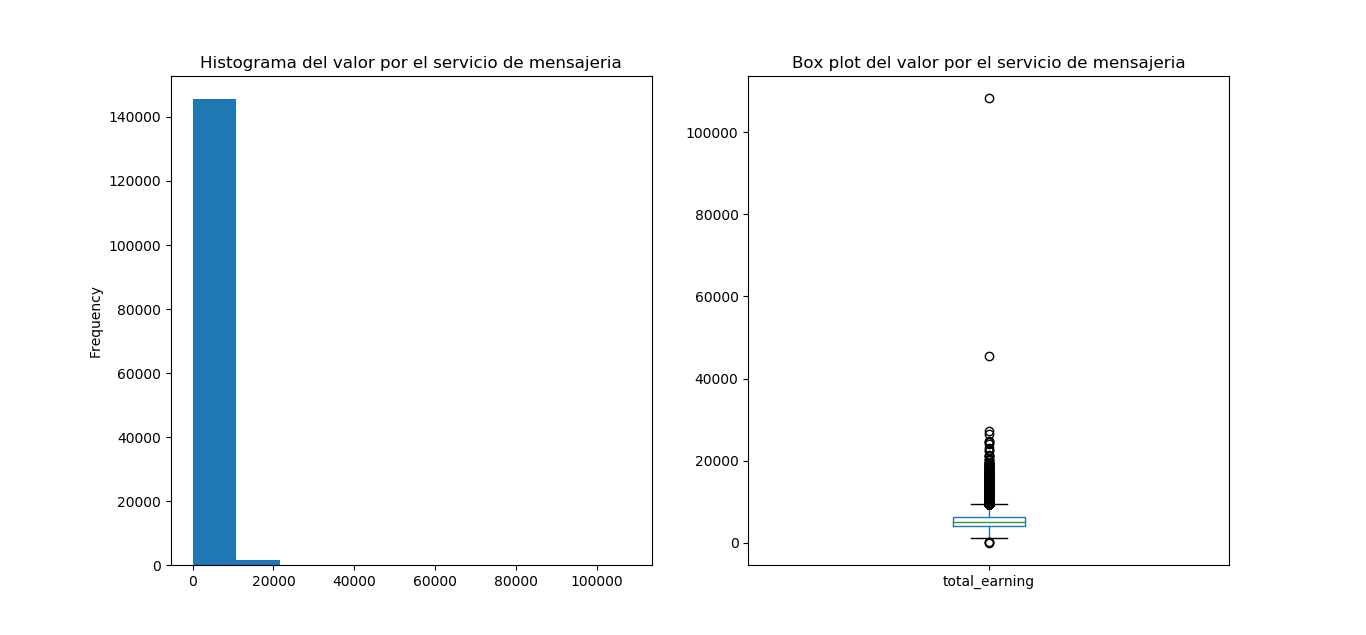
\includegraphics[width=0.5\textwidth]{../Img/total_earning}
		\end{figure}
	\section{Recomendaciones}
		Es claro que los días (lunes, martes, miércoles, jueves, viernes, sábado y domingo) no tienen mayor incidencia en la decisión de tomar o rechazar un servicio más allá de que a partir del día viernes y durante todo el fin de semana hay un incremento en los mismos.\\
		
		\begin{figure}[h]
			\centering
			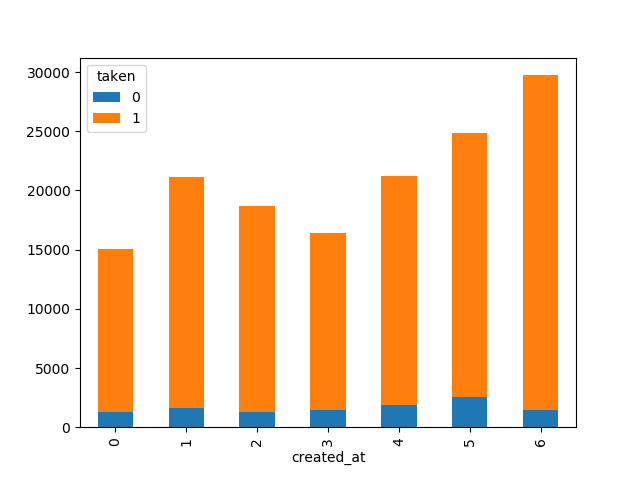
\includegraphics[width=0.5\textwidth]{../Img/Figure_2}
		\end{figure}
		El tema de las horas si es decisivo para dicha decisión. Es por eso que tomamos un prime time, un rango que va desde las 11 de la mañana hasta las 8 de la noche (22 horas). Esto con el fin de decir que si se encuentra en ese horario es muy probable que el servicio sea tomado.\\
		
		\begin{figure}[h]
			\centering
			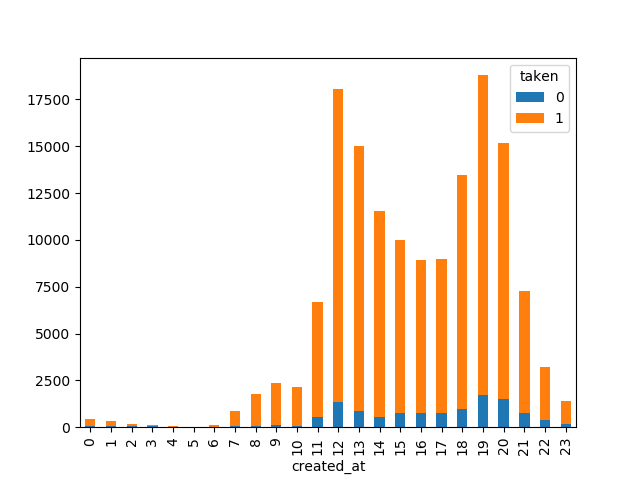
\includegraphics[width=0.5\textwidth]{../Img/Figure_3}
		\end{figure}
		Vemos como la altura no está correlacionada con la decisión de tomar o no el servicio. Pero si es evidente como a partir de una distancia de 1.5 kilómetros los servicios se empiezan a tomar como rechazados gran cantidad de servicios.\\
		
		\begin{figure}[h]
			\centering
			\includegraphics[width=0.5\textwidth]{../Img/Figure_6}
		\end{figure}
			
		\begin{figure}[h]
			\centering
			\includegraphics[width=0.5\textwidth]{../Img/Figure_7}
		\end{figure}
		El rango del valor es cerrado y no se evidencia ninguna corrección entre el valor ganado y la variable taken.
		\begin{figure}[h]
			\centering
			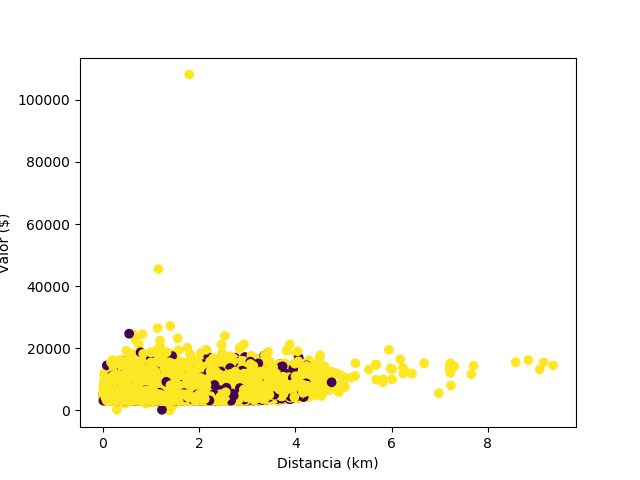
\includegraphics[width=0.5\textwidth]{../Img/Figure_5}
		\end{figure}
	\section{Modelo}	
		Se opto por un modelo logístico pues es un tipo de análisis de regresión utilizado para predecir el resultado de una variable categórica (una variable que puede adoptar un número limitado de categorías) en función de unas variables predictoras. Es útil para modelar la probabilidad de un evento ocurriendo como función de otros factores.\\
		
		\begin{figure}[h]
			\centering
			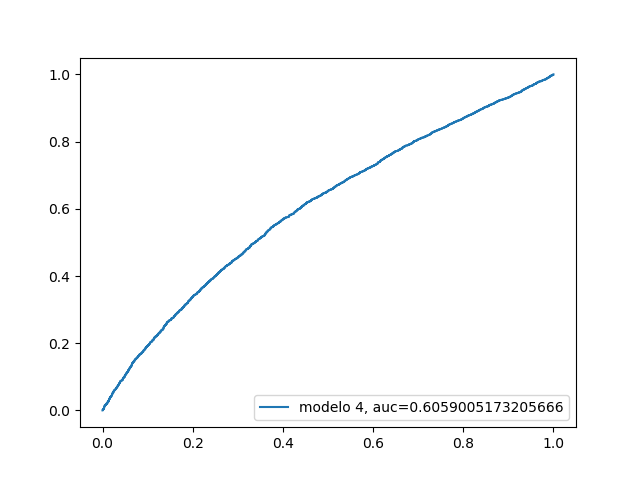
\includegraphics[width=0.5\textwidth]{../Img/curvaRocModelo4}
		\end{figure}
		Para nuestro modelo se tomaron como variables predictoras el rango prime time definido anteriormente \textit{primeTime} y la distancia (en km) entre la tienda y el usuario final. El modelo cuenta con una exactitud en la predicción del 92\% y una precisión del 92\%.
\end{document}